\documentclass{article}

% set font encoding for PDFLaTeX, XeLaTeX, or LuaTeX
\usepackage{ifxetex,ifluatex}
\newif\ifxetexorluatex
\ifxetex
  \xetexorluatextrue
\else
  \ifluatex
    \xetexorluatextrue
  \else
    \xetexorluatexfalse
  \fi
\fi

\ifxetexorluatex
  \usepackage{fontspec}
\else
  \usepackage[T1]{fontenc}
  \usepackage[utf8]{inputenc}
  \usepackage{lmodern}
\fi

\usepackage{hyperref}
\usepackage{graphicx}


\title{Actividad 9}
\author{Jesús Adrián Zatarain Alvarado}

% Enable SageTeX to run SageMath code right inside this LaTeX file.
% http://mirrors.ctan.org/macros/latex/contrib/sagetex/sagetexpackage.pdf
% \usepackage{sagetex}

\begin{document}
\maketitle

\section{Introducción}

A continuación se desplega un manual que resalta lo más importante para el uso básico de Maxima, y resaltando sus capacidades más notorias. Máxima es una herramienta muy útil para la realización de ćalculos y obtención de gráficas.

\section{¿Qué es Máxima?}

El sistema de álgebra computacional Maxima es un motor de cálculo simbólico escrito en lenguaje Lisp publicado bajo licencia GNU GPL.

Cuenta con un amplio conjunto de funciones para hacer manipulación simbólica de polinomios, matrices, funciones racionales, integración, derivación, manejo de gráficos en 2D y 3D, manejo de números de coma flotante muy grandes, expansión en series de potencias y de Fourier, entre otras funcionalidades. Además tiene un depurador a nivel de fuente para el código de Maxima.

Maxima está basado en el sistema original de Macsyma desarrollado por MIT en los años 70. Es bastante fiable, tiene un buen recolector de basura, por lo que no desperdicia memoria. Viene con cientos de auto pruebas (test-suite).

Maxima funciona en modo consola, sin embargo incluye las intefaces gráficas xMaxima y wxMaxima para facilitar su uso.

El editor de texto científico GNU TeXmacs también puede ser usado para facilitar una interfaz gráfica de usuario para Maxima. Otras opciones son, imaxima, y el modo interactivo de Emacs. También puede hacer uso de la interfaz gráfica de SageMath, que facilita su integración con otras herramientas CAS.

Como está escrito en Common Lisp, es fácilmente accesible para la programación, desde la capa inferior de Lisp puede llamarse a Maxima.

\section{Características}

\subsection{Entrada y salida}

Cuando se inicia una sesión de Maxima, aparecerá la etiqueta (porciento i1), que significa entrada 1. Se debe escribir un comando válido al lado de esa etiqueta, que termina con un punto y coma y cuando se pulsa la tecla Intro, esa entrada se analizará , simplificado, vinculado a una variable interna porciento i1 y su resultado se mostrará después de una etiqueta (porciento o1), que significa salida 1. Ese resultado también estará vinculado a una variable interna porciento o1. Aparecerá otra etiqueta (porciento i2) a continuación, para marcar el lugar donde debe escribirse un segundo comando y así sucesivamente. El uso más básico de Maxima es como una calculadora.


\subsection{Variables}

To link a value or other objects to a variable, the symbol ":" is used, and not the equal sign "=", which will be used to define mathematical equations. The name of the variables can be any combination of letters, numbers and one of the symbols porciento or _, but the first character cannot be a number.

Maxima configura varias variables internas, con nombres que empiezan por porciento. Algunos ejemplos son las variables porciento i2 y porciento o2, vinculadas a un comando de entrada y su resultado. El símbolo porciento en sí mismo representa el último resultado obtenido; por ejemplo, en la entrada porciento i19, habría sido suficiente escribir porciento en lugar de porciento o18.

Es más seguro no utilizar nombres de variables que ya están siendo utilizados por Maxima, aunque es posible usar el mismo nombre para una variable, una función y objetos de diferentes tipos.

Maxima simplifica la mayoría de los comandos de entrada antes de ejecutarlos. En este último ejemplo, como resultado de esa simplificación, las variables en el producto m * a se reordenaron alfabéticamente. Si cualquiera de las 3 variables en la ecuación, F, m y a estuvieran vinculadas a un valor, ese valor se habría reemplazado, y la segunda ley variable se vincularía a la ecuación obtenida después de esa sustitución y simplificación. En este caso, ninguna de las variables estaba vinculada a ningún valor; si más adelante una de las variables en la ecuación está vinculada al valor, la ecuación vinculada a la segunda ley sigue siendo la misma


\subsection{Listas}

Una variable también se puede vincular a una lista de valores, que se colocan entre corchetes y separados por comas. Muchas de las operaciones realizadas por Maxima entre los números también se pueden hacer entre listas

Una función muy útil para crear listas es makelist, que expande una expresión, reemplazando varios valores diferentes para una variable determinada. El primer argumento dado a makelist debe ser la expresión a expandir y el segundo argumento es el nombre de la variable que será reemplazada por una secuencia de valores desde un valor inicial hasta un valor máximo definido por el tercer y cuarto argumentos. Si se proporciona un quinto argumento, se usará como el incremento en la secuencia de valores que se reemplazarán; de lo contrario, se usará el incremento predeterminado de 1.

El tercer argumento dado a la función makelist también puede ser una lista con la secuencia de valores que debe reemplazarse para la variable en el segundo argumento.





\subsection{constantes}

Maxima acepta números reales y complejos. Los números reales en Maxima pueden ser enteros, racionales, como 3/5, o números de coma flotante, por ejemplo, 2.56 y 25.6e-1, que es una notación corta para 25.6 x 10-1. Los números irracionales, como sqrt (2) (raíz cuadrada de 2) o log (2) (logaritmo natural de 2) se dejan en esa forma, sin ser aproximados por números de coma flotante, y cálculos posteriores, como sqrt (2 )  2 o exp (log (2)) conducirá al resultado exacto 2.

Los números de coma flotante son "contagiosos"; es decir, las operaciones en las que ingresen se llevarán a cabo en ese formato. Por ejemplo, si en lugar de escribir log (2) uno escribiera log (2.0), el logaritmo se calcularía aproximadamente en coma flotante. Otra forma de forzar que una expresión se compute como un número de coma flotante consiste en usar la función flotante. Por ejemplo, dado que el resultado (porciento o2) obtenido anteriormente estaba vinculado a la variable porciento o2, para obtener una aproximación de coma flotante de ese resultado.

Una fuente frecuente de confusión surge del hecho de que esos números están siendo representados internamente en base binaria y no en base decimal; por lo tanto, ciertos números que pueden representarse en decimal con algunos dígitos, por ejemplo 0.1, necesitarían un número infinito de dígitos binarios para ser representados con precisión en base binaria. Es lo mismo que ocurre con la fracción 1/3 en base decimal, que en forma de coma flotante tiene un número infinito de dígitos: 0,333 ... (en el sistema base 3, esa fracción se puede representar fácilmente). Las fracciones que conducen a un número infinito de dígitos no son las mismas en los sistemas de base decimal y binario.

Hay algunas constantes matemáticas predefinidas en Maxima. Los nombres de variable vinculados a esas constantes generalmente comienzan con el símbolo porciento. Tres constantes importantes son el número, vinculado a porciento pi, el número de Euler, la base de los logaritmos naturales, vinculado a porciento ey el número imaginario, vinculado a porciento i.

Tanto porciento pi como porciento e son números irracionales que no se pueden representar exactamente con un número finito de dígitos, pero se puede obtener una aproximación de coma flotante, con 16 dígitos significativos, utilizando la función float; también se puede encontrar una representación numérica con dígitos más significativos utilizando la función bfloat y la variable fpprec.






\section{Gráficas}

\subsection{Parametrización de curvas y superficies}

plot2d se usa para mostrar la representación de una o varias funciones de una variable.
Para trazar varias funciones en la misma ventana, esas funciones se colocan dentro de una lista. Command plot3d se usa para trazar funciones de dos variables.



\section{Utilidades}

\subsection{álgebra}

Las expresiones pueden incluir operaciones matemáticas con variables abstractas


La variable x permanece indefinida, ya que el signo igual no vincula la variable con el valor del otro lado. Los resultados dados en (porciento o36) son aproximaciones numéricas y no las raíces exactas. En algunos casos, las expresiones algebraicas exactas para las raíces se pueden encontrar utilizando el comando resolver, que también puede resolver otros tipos de ecuaciones, no solo polinomios.


\subsection{Trigonometría}

Las funciones que esperan un ángulo como argumento de entrada interpretan ese ángulo en radianes y no en grados, ya que Maxima también conoce algunas propiedades de esas funciones, incluidas sus series de potencias, que solo son válidas cuando el ángulo se da en radianes.

el resultado fue exacto cuando el argumento dado a la función se escribió en forma exacta, usando un número racional. La función atan2 toma dos argumentos de entrada, que son las coordenadas cartesianas y de un punto, y devuelve un ángulo que puede estar en cualquiera de los 4 cuadrantes (entre pi y pi), y corresponde al ángulo entre el segmento desde el origen hasta ese punto y el semi-eje positivo Para convertir un ángulo de radianes a grados, se multiplica por 180 y se divide por pi.

Hay múltiples expresiones para simplificar o escribir identidades trigonométricas.

\begin{center}
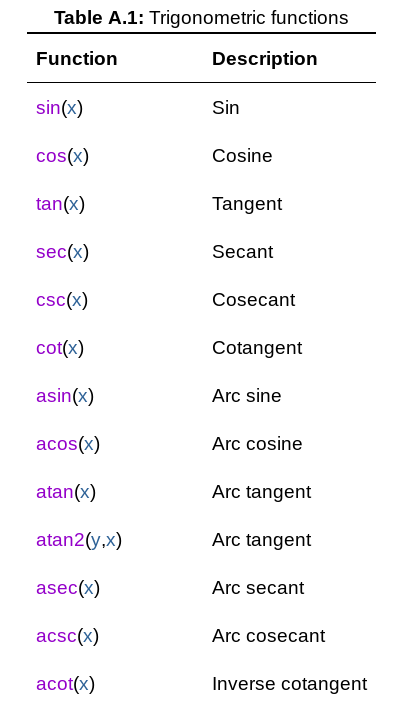
\includegraphics[width=6cm, height=6cm]{trig.png}

\end{center}

\subsection{Cálculo}

La forma más sencilla de representar funciones matemáticas en Maxima es mediante el uso de expresiones. Maxima también tiene su propia sintaxis para definir funciones generales, que es el tema de la siguiente sección, y que puede usarse en el caso de las funciones matemáticas.

El valor de la función en un punto se obtendría directamente, pero para calcular la derivada y antiderivada ahora es necesario escribir la función y la variable en su argumento.

\section{conclusión}

Maxima es una herramienta muy importante para el desarrollo de cálculos y obtención de gráficas. Tiene distintas bondades que lo hacen una herramienta muy amigable e intuitiva para poder desarrollar cualquier proyecto o tarea pedida a lo largo de la carrera.


\section{Apéndice}

1.- ¿Cuál fue tu primera impresión de Wxmaxima?
\\
\\
Una herramienta muy útil para realizar cálculos, con una interfaz muy amigable y muy dinámica.
\\
\\
2.- ¿Crees que esta herramienta puede ser útil en otros de tus cursos?
\\
\\
Es útil para hacer cálculos complejos y necesaria para cualquier curso en la carrera
\\
\\
3.- ¿Qué se te dificultó mas en esta actividad?
\\
\\
El recopilar la información de distintas fuentes
\\
\\
4.- ¿Se te hizo compleja esta actividad? ¿Cómo la mejorarías? 
\\
\\
No fue compleja, así está bien
\end{document}
